\chapter{哈恩-巴拿赫定理。共轭凸函数理论导论}
\section{哈恩-巴拿赫定理的解析形式:线性泛函的扩张}

设$E$是$\mathbb{R}$上的一个向量空间。我们回忆一下,一个\textbf{泛函}是定义在$E$上,或$E$的某个子空间上,取值为$\mathbb{R}$的函数。本节的主要结果涉及将定义在$E$的一个线性子空间上的线性泛函延拓为定义在整个$E$上的线性泛函。

\begin{theorem}[Helly, Hahn-Banach 解析形式]\label{theorem1.1}
设 $p: E \to \mathbb{R}$ 是一个满足以下条件的函数\footnote{一个满足(1)和(2)的函数有时被称为\textbf{闵可夫斯基泛函} (Minkowski functional)。}
\begin{enumerate}[(1)]
\item $p(\lambda x) = \lambda p(x) \quad \forall x \in E \text{ and } \forall \lambda > 0,$
\item $p(x+y) \leq p(x) + p(y) \quad \forall x, y \in E.$
\end{enumerate}
设 $G \subset E$ 是一个线性子空间,并设 $g: G \to \mathbb{R}$ 是一个线性泛函,使得
\begin{equation}\label{eq3}
g(x) \leq p(x) \quad \forall x \in G.
\end{equation}
在这些假设下,存在一个定义在整个$E$上的线性泛函$f$,它延拓了$g$,即 $g(x) = f(x) \quad \forall x \in G$,并且使得
\begin{equation}\label{eq4}
f(x) \leq p(x) \quad \forall x \in E.
\end{equation}
\end{theorem}

定理\ref{theorem1.1}的证明依赖于Zorn引理,这是一个著名的、非常有用的有序集的性质。在陈述Zorn引理之前,我们必须澄清一些概念。设$P$是一个带有(偏)序关系$\leq$的集合。我们说一个子集$Q \subset P$是\textbf{全序的} (totally ordered),如果对于任何一对$(a, b) \in Q$,或者$a \leq b$或者$b \leq a$(或者两者都成立!)。设$Q \subset P$是$P$的一个子集;我们说$c \in P$是$Q$的一个\textbf{上界} (upper bound),如果对于每一个$a \in Q$都有$a \leq c$。我们说$m \in P$是$P$的一个\textbf{极大元} (maximal element),如果不存在$x \in P$使得$m \leq x$且$x \neq m$。注意,$P$的极大元不一定是$P$的上界。我们说$P$是\textbf{归纳的} (inductive),如果$P$中的每个全序子集$Q$都有一个上界。

\begin{lemma}[Zorn]\label{lemma1.1}
每个非空归纳集都有一个极大元。
\end{lemma}

Zorn引理源于选择公理,但我们不讨论它的推导;参见,例如,J. Dugundji [1], N. Dunford-J. T. Schwartz [1] (Volume 1, Theorem 1.2.7), E. Hewitt-K. Stromberg [1], S. Lang [1], and A. Knapp [1]。

\begin{remark}
Zorn引理在分析中有许多重要的应用。它是在一些看似无害的存在性陈述中非常有用的工具,例如“每个向量空间都有一个基底”(见练习1.5)和“在任何向量空间上都存在非平凡的线性泛函”。大多数分析学家不知道如何证明Zorn引理;但对于一个分析学家来说,能够理解Zorn引理的陈述并正确使用它,是非常重要的。
\end{remark}

\begin{proof}
考虑集合
\[ P = \left\{ h: D(h) \to \mathbb{R} \;\middle|\; \begin{array}{l} D(h) \text{是E的线性子空间, } G \subset D(h) \\ h \text{ 是线性的, 延拓 } g, \text{且} \\ h(x) \leq p(x) \quad \forall x \in D(h) \end{array} \right\}. \]
在$P$上我们定义序关系
\[ (h_1 \leq h_2) \Leftrightarrow (D(h_1) \subset D(h_2) \text{ 且 } h_2 \text{ 延拓 } h_1). \]
很明显$P$是非空的,因为$g \in P$。我们断言$P$是归纳的。实际上,设$Q \subset P$是一个全序子集;我们记$Q = (h_i)_{i \in I}$并设
\[ D(h) = \bigcup_{i \in I} D(h_i), \quad h(x) = h_i(x) \quad \text{如果 } x \in D(h_i) \text{ 对于某个 } i. \]
很容易看出$h$的定义是合理的,即$h \in P$,并且$h$是$Q$的一个上界。我们可以应用Zorn引理,因此我们有一个极大元$f$。我们断言$D(f) = E$,这样就完成了证明。
假设,与此相反,$D(f) \neq E$。设$x_0 \notin D(f)$;设$D(h) = D(f) + \mathbb{R}x_0$,并且对于每一个$x \in D(f)$和$t \in \mathbb{R}$,我们定义$h(x+tx_0) = f(x) + t\alpha$,其中常数$\alpha \in \mathbb{R}$将被选择,使得$h \in P$。我们必须确保
\[ f(x) + t\alpha \leq p(x+tx_0) \quad \forall x \in D(f) \quad \text{且} \quad \forall t \in \mathbb{R}. \]
鉴于(1),这等价于对 $\forall x \in D(f)$ 有
\begin{align*}
f(x) + \alpha &\leq p(x+x_0) \\
f(x) - \alpha &\leq p(x-x_0)
\end{align*}
换句话说,我们必须找到一个满足条件的$\alpha$,即
\[ \sup_{y \in D(f)} \{f(y) - p(y-x_0)\} \leq \alpha \leq \inf_{x \in D(f)} \{p(x+x_0) - f(x)\}. \]
这样的$\alpha$是存在的,因为 $\forall x \in D(f), \forall y \in D(f)$,有
\[ f(y) - p(y-x_0) \leq p(x+x_0) - f(x); \]
实际上,这由(2)可得
\[ f(x)+f(y) \leq p(x+y) \leq p(x+x_0) + p(y-x_0). \]
我们得出$f \leq h$;但这是不可能的,因为$f$是极大的且$h \neq f$。
\end{proof}

我们现在描述定理\ref{theorem1.1}的一些简单应用,其中$E$是一个范数向量空间(n.v.s.),其范数为$\| \cdot \|$。

我们用$E^*$表示$E$的对偶空间,即$E$上所有\textbf{连续}线性泛函的空间;$E^*$上的(对偶)范数定义为
\begin{equation}\label{eq5}
\|f\|_{E^*} = \sup_{\|x\| \leq 1} |f(x)| = \sup_{\|x\|=1} |f(x)|.
\end{equation}
在没有歧义的情况下,我们也将写作$\|f\|$而不是$\|f\|_{E^*}$。给定$f \in E^*$和$x \in E$,我们将写作$\langle f, x \rangle$而不是$f(x)$;我们说$\langle \cdot, \cdot \rangle$是$E^*$和$E$之间的\textbf{对偶内积}。众所周知,$E^*$是一个Banach空间,即$E^*$是完备的(即使$E$不是);这源于$\mathbb{R}$是完备的这一事实。

\begin{corollary}\label{corollary1.2}
设$G \subset E$是一个线性子空间。如果$g: G \to \mathbb{R}$是一个连续线性泛函,那么存在一个$f \in E^*$,它延拓$g$并且使得
\[ \|f\|_{E^*} = \|g\|_{G^*} = \sup_{\substack{x \in G, \\ \|x\| \leq 1}} |g(x)|. \]
\end{corollary}
\begin{proof}
使用定理\ref{theorem1.1},其中$p(x) = \|g\|_{G^*} \|x\|$。
\end{proof}

\begin{corollary}\label{corollary1.3}
对于每个$x_0 \in E$,存在一个$f_0 \in E^*$使得
\[ \|f_0\|_{E^*} = \|x_0\| \quad \text{且} \quad \langle f_0, x_0 \rangle = \|x_0\|^2. \]
\end{corollary}
\begin{proof}
使用推论\ref{corollary1.2},其中$G=\mathbb{R}x_0$且$g(tx_0) = t\|x_0\|^2$,所以$\|g\|_{G^*} = \|x_0\|$。
\end{proof}

\begin{remark}
由推论\ref{corollary1.3}给出的元素$f_0$通常不是唯一的(尝试构造一个例子或见练习1.2)。然而,如果$E^*$是\textbf{严格凸的}\footnote{如果对所有$t \in (0,1)$,以及所有$y, v$满足$\|y\|=\|v\|=1$和$y \neq v$,都有$\|ty+(1-t)v\| < 1$,则称赋范空间是\textbf{严格凸}的;见练习1.26。}(例如,如果$E$是一个Hilbert空间(见第五章)或$E = L^p(\Omega)$,其中$1 < p < \infty$),那么$f_0$是唯一的。然而,在一般情况下,对于每个$x_0 \in E$,集合
\[ F(x_0) = \{f_0 \in E^* : \|f_0\| = \|x_0\| \text{ 且 } \langle f_0, x_0 \rangle = \|x_0\|^2 \} \]
是(多值)映射$x_0 \mapsto F(x_0)$,称为从$E$到$E^*$的\textbf{对偶映射} (duality map);它的一些性质在练习1.1、1.2、3.28和问题13中有所描述。
\end{remark}

\begin{corollary}\label{corollary1.4}
对于每个$x \in E$,我们有
\begin{equation}\label{eq6}
\|x\| = \sup_{\substack{f \in E^* \\ \|f\| \leq 1}} \langle f, x \rangle = \max_{\substack{f \in E^* \\ \|f\| \leq 1}} |\langle f, x \rangle|.
\end{equation}
\end{corollary}
\begin{proof}
我们总可以假设$x \neq 0$。很明显
\[ \sup_{\substack{f \in E^* \\ \|f\| \leq 1}} |\langle f, x \rangle| \leq \|x\|. \]
另一方面,由推论\ref{corollary1.3},我们知道存在$f_0 \in E^*$使得$\|f_0\| = \|x\|$且$\langle f_0, x \rangle = \|x\|^2$。设$f_1 = f_0/\|x\|$,那么$\|f_1\| = 1$且$\langle f_1, x \rangle = \|x\|$。
\end{proof}

\begin{remark}
公式\eqref{eq5}——这是一个\textbf{定义}——不应与公式\eqref{eq6}混淆,后者是一个\textbf{陈述}。一般来说,\eqref{eq5}中的“sup”是无法达到的;参见,例如,练习1.3。然而,当$E$是自反的Banach空间时,\eqref{eq5}中的“sup”是可以达到的(见第三章);R. C. James断言的一个深刻结果是,如果$E$是一个Banach空间,使得对于每个$f \in E^*$,\eqref{eq5}中的sup是可以达到的,那么$E$是自反的;参见,例如,J. Diestel [1, Chapter 1]或R. Holmes [1]。
\end{remark}

\section{哈恩-巴拿赫定理的几何形式:凸集的分离}
我们从关于超平面的一些初步事实开始。在下文中,$E$表示一个赋范向量空间(n.v.s.)。

\begin{definition}
一个\textbf{仿射超平面} (affine hyperplane)是$E$的一个子集$H$,形式为
\[ H = \{x \in E; f(x) = \alpha\}, \]
其中$f$是一个不恒为零的线性泛函\footnote{我们不假设$f$是连续的(在无限维赋范空间中存在不连续的线性泛函;见练习1.5)。},$\alpha \in \mathbb{R}$是一个给定的常数。我们写$H=[f=\alpha]$,并称$f=\alpha$是$H$的方程。
\end{definition}

\begin{proposition}\label{proposition1.5}
超平面 $H = [f = \alpha]$ 是闭集当且仅当$f$是连续的。
\end{proposition}
\begin{proof}
如果$f$是连续的,则$H$是闭集是显然的。反之,我们假设$H$是闭集。$H$的补集$H^c$是开集且非空(因为$f$不恒为零)。设$x_0 \in H^c$,所以$f(x_0) \neq \alpha$,例如$f(x_0) < \alpha$。固定$r > 0$使得$B(x_0, r) \subset H^c$,其中
\[ B(x_0, r) = \{x \in E; \|x-x_0\| < r \}. \]
我们断言
\begin{equation}\label{eq7}
f(x) < \alpha \quad \forall x \in B(x_0, r).
\end{equation}
事实上,通过矛盾来证明。假设存在某个$x_1 \in B(x_0, r)$使得$f(x_1) > \alpha$。线段
\[ \{x_t = (1-t)x_0 + tx_1; t \in [0, 1]\} \]
包含在$B(x_0, r)$中,因此也在$H^c$中,所以$f(x_t) \neq \alpha, \forall t \in [0, 1]$;另一方面,$f(x_t) = \alpha$对于$t = \frac{\alpha - f(x_0)}{f(x_1) - f(x_0)} \in (0, 1)$,这是一个矛盾,因此\eqref{eq7}得证。它源于\eqref{eq7}
\[ f(x_0+rz) < \alpha \quad \forall z \in B(0, 1). \]
因此,$f$是连续的,并且$\|f\| \leq \frac{1}{r}(\alpha - f(x_0))$。
\end{proof}

\begin{definition}
设$A$和$B$是$E$的两个子集。我们称超平面$H = [f=\alpha]$ \textbf{分离} (separates) $A$和$B$,如果
\[ f(x) \leq \alpha \quad \forall x \in A \quad \text{且} \quad f(x) \geq \alpha \quad \forall x \in B. \]
我们说$H$ \textbf{严格分离} (strictly separates) $A$和$B$,如果存在$\varepsilon > 0$使得
\[ f(x) \leq \alpha - \varepsilon \quad \forall x \in A \quad \text{且} \quad f(x) \geq \alpha + \varepsilon \quad \forall x \in B. \]
\end{definition}
几何上,分离意味着$A$位于由$H$确定的一个半空间中,而$B$位于另一个半空间中;见图\ref{fig:1}。最后,我们回忆一下,如果对于任意$x,y \in A$,对于所有$t \in [0,1]$,都有$tx+(1-t)y \in A$,那么子集$A \subset E$是\textbf{凸的} (convex)。

\begin{figure}[H]
    \centering
    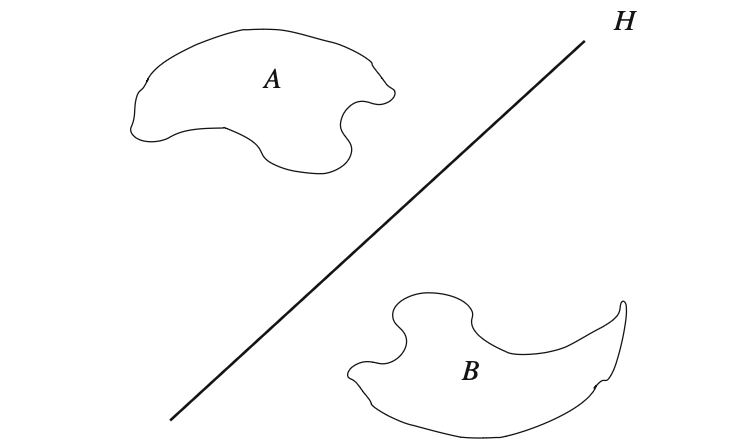
\includegraphics[width=0.8\textwidth]{image/fig1.png}
    \caption{图1:超平面$H$分离集合$A$和$B$。}
    \label{fig:1}
\end{figure}

\begin{theorem}[Hahn-Banach,第一几何形式]\label{theorem1.6}
设$A \subset E$和$B \in E$是两个非空不相交的凸子集,即$A \cap B = \emptyset$。假设其中一个是开集。那么存在一个闭超平面分离$A$和$B$。
\end{theorem}

定理\ref{theorem1.6}的证明依赖于下面两个引理。

\begin{lemma}\label{lemma1.2}
设$C \subset E$是一个包含$0$的开凸集。对于每个$x \in E$设
\begin{equation}\label{eq8}
p(x) = \inf\{\alpha > 0; \alpha^{-1}x \in C\}
\end{equation}
($p$被称为$C$的\textbf{规范} (gauge)或$C$的\textbf{闵可夫斯基泛函} (Minkowski functional))。
那么$p$满足(1),(2),并且
\begin{gather}
\text{存在一个常数 } M \text{ 使得 } 0 \leq p(x) \leq M\|x\| \quad \forall x \in E, \label{eq9} \\
C = \{x \in E; p(x) < 1\}. \label{eq10}
\end{gather}
\end{lemma}
\begin{proof}
(1)成立是显然的。

\eqref{eq9}的证明。设$r>0$使得$B(0, r) \subset C$;我们显然有
\[ p(x) \leq \frac{1}{r}\|x\| \quad \forall x \in E. \]

\eqref{eq10}的证明。首先,假设$x \in C$;因为$C$是开集,所以对于$\varepsilon>0$足够小,有$(1+\varepsilon)x \in C$,因此$p(x) \leq \frac{1}{1+\varepsilon} < 1$。反之,如果$p(x) < 1$,则存在$\alpha \in (0, 1)$使得$\alpha^{-1}x \in C$,因此$x = \alpha(\alpha^{-1}x) + (1-\alpha)0 \in C$。
设$x, y \in E$和$\varepsilon > 0$。使用(1)和(10)我们得到$\frac{x}{p(x)+\varepsilon} \in C$且$\frac{y}{p(y)+\varepsilon} \in C$。因此$t\frac{x}{p(x)+\varepsilon} + (1-t)\frac{y}{p(y)+\varepsilon} \in C$对于所有$t \in [0, 1]$成立。选择$t=\frac{p(x)+\varepsilon}{p(x)+p(y)+2\varepsilon}$,我们发现$\frac{x+y}{p(x)+p(y)+2\varepsilon} \in C$。再次使用(1)和(10),我们得到$p(x+y) < p(x)+p(y)+2\varepsilon, \forall \varepsilon > 0$。
\end{proof}

\begin{lemma}\label{lemma1.3}
设$C \subset E$是一个非空开凸集,并设$x_0 \in E$且$x_0 \notin C$。那么存在$f \in E^*$使得$f(x) < f(x_0)$对于所有$x \in C$成立。特别地,超平面$[f = f(x_0)]$分离$\{x_0\}$和$C$。
\end{lemma}
\begin{proof}
经过平移,我们可以假设$0 \in C$。我们可以引入$C$的规范$p$(见引理\ref{lemma1.2})。考虑线性子空间$G = \mathbb{R}x_0$和线性泛函$g: G \to \mathbb{R}$,定义为
\[ g(tx_0) = t, \quad t \in \mathbb{R}. \]
很明显
\[ g(x) \leq p(x) \quad \forall x \in G \]
(考虑$t>0$和$t<0$两种情况)。从定理\ref{theorem1.1}可知,存在一个延拓$g$并满足
\[ f(x) \leq p(x) \quad \forall x \in E. \]
的线性泛函$f$。
特别地,我们有$f(x_0)=1$并且$f$是连续的。我们从\eqref{eq10}推断出,对于每个$x \in C$,$f(x) < 1$。
\end{proof}

\begin{proof}
设$C=A-B = \bigcup_{y \in B} (A-y)$,那么$C$是凸的(检查!),$C$是开的(因为$C=\bigcup_{y \in B}(A-y)$),并且$0 \notin C$(因为$A \cap B = \emptyset$)。由引理\ref{lemma1.3}可知,存在某个$f \in E^*$使得
\[ f(z) < 0 \quad \forall z \in C, \]
即,
\[ f(x) < f(y) \quad \forall x \in A, \quad \forall y \in B. \]
固定一个常数$\alpha$满足
\[ \sup_{x \in A} f(x) \leq \alpha \leq \inf_{y \in B} f(y). \]
显然,超平面$[f=\alpha]$分离$A$和$B$。
\end{proof}

\begin{theorem}[Hahn-Banach,第二几何形式]\label{theorem1.7}
设$A \subset E$和$B \subset E$是两个非空不相交的凸子集。假设$A$是闭集,$B$是紧集。那么存在一个严格分离$A$和$B$的闭超平面。
\end{theorem}
\begin{proof}
设$C=A-B$,那么$C$是凸的,闭的(检查!),并且$0 \notin C$。因此,存在某个$r>0$使得$B(0,r) \cap C = \emptyset$。由定理\ref{theorem1.6}可知,存在一个分离$B(0,r)$和$C$的闭超平面。因此存在某个$f \in E^*, f \neq 0$使得
\[ f(x-y) \leq f(z) \quad \forall x \in A, \quad \forall y \in B, \quad \forall z \in B(0,1). \]
因此$f(x-y) \leq -r\|f\|$对于所有$x \in A, y \in B$成立。令$\varepsilon = \frac{1}{2}r\|f\| > 0$,我们得到
\[ f(x) + \varepsilon \leq f(y) - \varepsilon \quad \forall x \in A, \quad \forall y \in B. \]
选择$\alpha$使得
\[ \sup_{x \in A} f(x) + \varepsilon \leq \alpha \leq \inf_{y \in B} f(y) - \varepsilon, \]
我们看到超平面$[f=\alpha]$严格分离$A$和$B$。
\end{proof}

\begin{remark}
假设$A \subset E$和$B \subset E$是两个非空不相交的凸集。如果我们不做进一步的假设,通常不可能分离$A$和$B$为一个闭超平面。甚至可以构造一个例子,其中$A$和$B$都是闭集(见练习1.14)。然而,如果$E$是有限维的,则总可以分离任意两个非空不相交的凸集$A$和$B$(无需进一步假设!);见练习1.9。
\end{remark}

我们以一个非常有用的事实来结束。
\begin{corollary}\label{corollary1.8}
设$F \subset E$是一个线性子空间,使得$\bar{F} \neq E$。那么存在$f \in E^*, f \neq 0$使得
\[ \langle f, x \rangle = 0 \quad \forall x \in F. \]
\end{corollary}
\begin{proof}
设$x_0 \in E$且$x_0 \notin \bar{F}$。使用定理\ref{theorem1.7},其中$A=\bar{F}$,$B=\{x_0\}$,我们发现一个闭超平面$[f=\alpha]$严格分离$\bar{F}$和$\{x_0\}$。因此,我们有
\[ \langle f, x \rangle < \alpha < \langle f, x_0 \rangle \quad \forall x \in \bar{F}. \]
由此可知$\langle f, x \rangle = 0$对于所有$x \in F$成立,因为$\lambda x \in F$,所以$\langle f, \lambda x \rangle < \alpha$对于所有$\lambda \in \mathbb{R}$成立。
\end{proof}

\begin{remark}
推论\ref{corollary1.8}在证明一个线性子空间$F \subset E$是稠密的时候非常有用。只需证明每个在$F$上处处为零的连续线性泛函都必须在$E$上处处为零。
\end{remark}

\section{对偶空间 $E^{**}$,正交关系}
设$E$是一个范数向量空间(n.v.s.),设$E^*$是其范数为
\[ \|f\|_{E^*} = \sup_{\substack{x \in E \\ \|x\| \leq 1}} |\langle f, x \rangle|. \]
的对偶空间。
对偶空间$E^{**}$是$E^*$的对偶空间,其范数为
\[ \|\xi\|_{E^{**}} = \sup_{\substack{f \in E^* \\ \|f\| \leq 1}} |\langle \xi, f \rangle| \quad (\xi \in E^{**}). \]
有一个\textbf{典范注入} (canonical injection) $J: E \to E^{**}$定义如下:给定$x \in E$,映射$f \mapsto \langle f, x \rangle$是$E^*$上的一个连续线性泛函;因此它是$E^{**}$中的一个元素,我们用$J_x$表示。\footnote{$J$不应与注记2中定义的对偶映射$F: E \to E^*$混淆。}我们有
\[ \langle Jx, f \rangle_{E^{**}, E^*} = \langle f, x \rangle_{E^*, E} \quad \forall x \in E, \quad \forall f \in E^*. \]
很明显,$J$是线性的,并且它是一个\textbf{等距同构} (isometry),即$\|Jx\|_{E^{**}} = \|x\|_{E}$;事实上,我们有
\[ \|Jx\|_{E^{**}} = \sup_{\substack{f \in E^* \\ \|f\| \leq 1}} |\langle Jx, f \rangle| = \sup_{\substack{f \in E^* \\ \|f\| \leq 1}} |\langle f, x \rangle| = \|x\| \]
(由推论\ref{corollary1.4})。
它可能发生$J$不是从$E$到$E^{**}$的\textbf{满射} (surjective)(见第三章和第四章)。然而,$J$的像$J(E)$是$E^{**}$的一个子空间。如果$J$是满射,我们就说$E$是\textbf{自反的} (reflexive),并且$E^{**}$与$E$等同(见第三章)。


如果$M \subset E$是一个线性子空间,我们设
\[ M^\perp = \{f \in E^*; \langle f, x \rangle = 0 \quad \forall x \in M\}. \]
如果$N \subset E^*$是一个线性子空间,我们设
\[ N^\perp = \{x \in E; \langle f, x \rangle = 0 \quad \forall f \in N\}. \]
注意——根据定义——$N^\perp$是$E$的一个子集,而不是$E^{**}$。很明显,$M^\perp$(相应地$N^\perp$)是$E^*$(相应地$E$)的闭线性子空间。我们说$M^\perp$(相应地$N^\perp$)是$M$(相应地$N$)的\textbf{正交补} (space orthogonal)。

\begin{proposition}\label{proposition1.9}
设$M \subset E$是一个线性子空间。则
\[ (M^\perp)^\perp = \bar{M}. \]
\end{proposition}
\begin{proof}
很明显$M \subset (M^\perp)^\perp$,并且由于$(M^\perp)^\perp$是闭的,我们有$\bar{M} \subset (M^\perp)^\perp$。反之,设$x_0 \in (M^\perp)^\perp$使得$x_0 \notin \bar{M}$。根据定理\ref{theorem1.7},存在一个闭超平面严格分离$\{x_0\}$和$\bar{M}$。因此存在一些$f \in E^*$和$\alpha \in \mathbb{R}$使得
\[ \langle f, x \rangle < \alpha < \langle f, x_0 \rangle \quad \forall x \in \bar{M}. \]
因为$M$是一个线性空间,所以$\langle f, x \rangle = 0 \quad \forall x \in M$,并且$\langle f, x_0 \rangle > 0$。因此$f \in M^\perp$,因此$\langle f, x_0 \rangle = 0$,这是一个矛盾。因此我们断定$N \subset (N^\perp)^\perp$。
\end{proof}

\begin{remark}
可能发生$N$严格大于$\bar{N}$(见练习1.16)。然而,尝试证明$(N^\perp)^\perp = \bar{N}$并找出论证的破绽是有启发性的。假设$f_0 \in E^*$使得$f_0 \in (N^\perp)^\perp$且$f_0 \notin \bar{N}$。应用Hahn-Banach(在$E^*$上),我们可以严格分离$\{f_0\}$和$\bar{N}$。因此,存在某个$\xi \in E^{**}$使得$\langle \xi, f_0 \rangle > 0$。但是我们不能推导出矛盾,因为$\xi \notin N^\perp$——除非我们碰巧知道(!)$\xi \in E$,或者更准确地说,$\xi=J x_0$对于某个$x_0 \in E$。特别地,如果$E$是自反的,那么$(N^\perp)^\perp = \bar{N}$确实成立。在一般情况下,可以证明$(N^\perp)^\perp$与$N$在弱$*$拓扑$\sigma(E^*, E)$中的闭包一致(见第三章)。
\end{remark}

\section{共轭凸函数理论简介}\label{sec:conjugate_convex}
我们从下半连续函数和凸函数的一些基本事实开始。在本节中,我们考虑定义在集合$E$上取值为$(-\infty, +\infty]$的函数$\varphi$,因此$\varphi$可以取值$+\infty$(但$-\infty$被排除)。我们用$D(\varphi)$表示$\varphi$的\textbf{定义域} (domain),即,
\[ D(\varphi) = \{x \in E; \varphi(x) < +\infty\}. \]
\paragraph{记号} $\varphi$的\textbf{上镜图} (epigraph)是集合\footnote{我们坚持$\mathbb{R} = (-\infty, \infty)$,所以$\lambda$不取值$\infty$。}
\[ \text{epi } \varphi = \{[x, \lambda] \in E \times \mathbb{R}; \varphi(x) \leq \lambda\}. \]
我们现在假设$E$是一个拓扑空间。我们回忆以下内容。
\begin{definition}
一个函数$\varphi: E \to (-\infty, +\infty]$被称为\textbf{下半连续的} (lower semicontinuous) (l.s.c.),如果对于每个$\lambda \in \mathbb{R}$,集合
\[ [\varphi \leq \lambda] = \{x \in E; \varphi(x) \leq \lambda\} \]
是闭集。
\end{definition}
这里有一些关于l.s.c.函数的著名的基本事实(见,例如,G. Choquet [1], J. Dixmier [1], J. R. Munkres [1], H. L. Royden [1]):
\begin{enumerate}
    \item 如果$\varphi$是l.s.c.的,那么它的上镜图在$E \times \mathbb{R}$中是闭集;反之亦然。
    \item 如果$\varphi$是l.s.c.的,那么对于每个$x \in E$和每个$\varepsilon > 0$,存在$x$的一个邻域$V$使得
    \[ \varphi(y) \geq \varphi(x) - \varepsilon \quad \forall y \in V; \]
    反之亦然。特别地,如果$\varphi$是l.s.c.的,那么对于$E$中的每个序列$(x_n)$,如果$x_n \to x$,我们有
    \[ \liminf_{n\to\infty} \varphi(x_n) \geq \varphi(x) \]
    如果$E$是度量空间,反之亦然。
    \item 如果$\varphi_1$和$\varphi_2$是l.s.c.的,那么$\varphi_1 + \varphi_2$也是l.s.c.的。
    \item 如果$(\varphi_i)_{i \in I}$是一族l.s.c.函数,那么它们的上包络线,即由
    \[ \varphi(x) = \sup_{i \in I} \varphi_i(x) \]
    定义的函数,也是l.s.c.的。
    \item 如果$E$是紧的且$\varphi$是l.s.c.的,那么$\inf_E \varphi$是可以达到的。
    (如果$E$是一个紧度量空间,人们可以用极小化序列来论证。对于一般的拓扑紧空间,考虑集合$[\varphi \leq \lambda]$对于适当的$\lambda$值。)
\end{enumerate}
我们现在假设$E$是一个向量空间。回忆以下定义。
\begin{definition}
一个函数$\varphi: E \to (-\infty, +\infty]$被称为\textbf{凸的} (convex),如果
\[ \varphi(tx+(1-t)y) \leq t\varphi(x) + (1-t)\varphi(y) \quad \forall x, y \in E, \quad \forall t \in (0, 1). \]
\end{definition}
我们应使用一些凸函数的基本性质:
\begin{enumerate}
    \item 如果$\varphi$是一个凸函数,那么上镜图$\text{epi } \varphi$是$E \times \mathbb{R}$中的一个凸集;反之亦然。
    \item 如果$\varphi$是一个凸函数,那么对于每个$\lambda \in \mathbb{R}$,集合$[\varphi \leq \lambda]$是凸集;但反之不成立。
    \item 如果$\varphi_1$和$\varphi_2$是凸函数,那么$\varphi_1 + \varphi_2$也是凸函数。
    \item 如果$(\varphi_i)_{i \in I}$是一族凸函数,那么上包络线$\sup_i \varphi_i$是凸的。
\end{enumerate}
我们此后假设$E$是一个n.v.s.。
\begin{definition}
设$\varphi: E \to (-\infty, +\infty]$是一个函数,使得$\varphi \not\equiv +\infty$(即$D(\varphi) \neq \emptyset$)。我们定义\textbf{共轭函数} (conjugate function) $\varphi^*: E^* \to (-\infty, +\infty]$为\footnote{$\varphi^*$有时被称为$\varphi$的\textbf{勒让德变换} (Legendre transform)。}
\[ \varphi^*(f) = \sup_{x \in E} \{\langle f, x \rangle - \varphi(x)\} \quad (f \in E^*). \]
\end{definition}
注意$\varphi^*$在$E^*$上是凸的且l.s.c.的。事实上,对于每个固定的$x \in E$,函数$f \mapsto \langle f, x \rangle - \varphi(x)$是凸的(实际上是仿射的)和连续的。它遵循这些函数的上包络线(当$x$遍历$E$时)是凸的且l.s.c.的。

\begin{figure}[H]
    \centering
    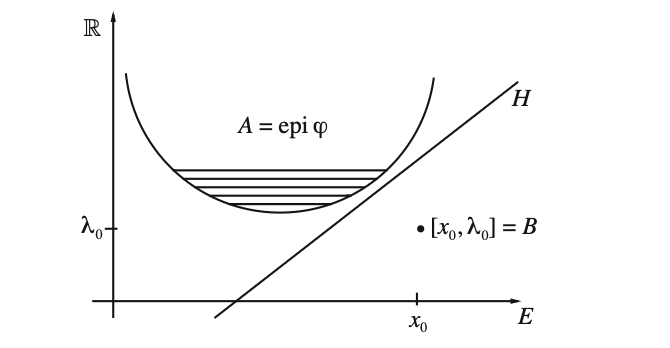
\includegraphics[width=0.8\textwidth]{image/fig2.png}
    \caption{图2}
    \label{fig:2}
\end{figure}

\begin{remark}
显然我们有不等式
\begin{equation}\label{eq11}
\langle f, x \rangle \leq \varphi(x) + \varphi^*(f) \quad \forall x \in E, \quad \forall f \in E^*,
\end{equation}
这有时被称为\textbf{杨氏不等式} (Young's inequality)。当然,这对于$\varphi$的定义是显而易见的!杨氏不等式的经典形式(见第四章定理4.6的证明)断言
\begin{equation}\label{eq12}
ab \leq \frac{1}{p}a^p + \frac{1}{p'}b^{p'} \quad \forall a, b \geq 0
\end{equation}
其中$1 < p < \infty$且$\frac{1}{p}+\frac{1}{p'}=1$。不等式\eqref{eq12}成为\eqref{eq11}的一个特例,其中$E=\mathbb{R}$且$\varphi(t)=\frac{1}{p}|t|^p, \varphi^*(s) = \frac{1}{p'}|s|^{p'}$(见练习1.18, 问题(h))。
\end{remark}

\begin{proposition}\label{proposition1.10}
假设$\varphi: E \to (-\infty, +\infty]$是凸的,l.s.c.的,且$\varphi \not\equiv +\infty$。那么$\varphi^* \not\equiv +\infty$,并且特别地,$\varphi$由一个仿射连续函数从下方有界。
\end{proposition}
\begin{proof}
设$x_0 \in D(\varphi)$并令$\varphi(x_0) < \lambda_0$。我们应用Hahn-Banach(第二几何形式)在空间$E \times \mathbb{R}$中,其中$A = \text{epi } \varphi$,$B = \{[x_0, \lambda_0]\}$。因此,存在一个严格分离$A$和$B$的闭超平面$H=[\Phi=\alpha]$ in $E \times \mathbb{R}$。注意,$\Phi$在$E \times \mathbb{R}$上的每个连续线性泛函都具有形式$\Phi([x, \lambda]) = \langle f, x \rangle + k\lambda$对于某个$f \in E^*$。令$k=\Phi([0,1])$,我们有
\[ \Phi([x, \lambda]) = \langle f, x \rangle + k\lambda \quad \forall [x, \lambda] \in E \times \mathbb{R}. \]
在$A$上写$\Phi > \alpha$,在$B$上写$\Phi < \alpha$,我们得到
\[ \langle f, x \rangle + k\lambda > \alpha \quad \forall [x, \lambda] \in \text{epi } \varphi, \]
和
\[ \langle f, x_0 \rangle + k\lambda_0 < \alpha. \]
特别地,我们有
\begin{equation}\label{eq13}
\langle f, x \rangle + k\varphi(x) > \alpha \quad \forall x \in D(\varphi)
\end{equation}
因此
\[ \langle f, x_0 \rangle + k\varphi(x_0) > \alpha > \langle f, x_0 \rangle + k\lambda_0. \]
它遵循$k>0$。由\eqref{eq13}我们有
\[ \langle -\frac{1}{k}f, x \rangle - \varphi(x) < -\frac{\alpha}{k} \quad \forall x \in D(\varphi) \]
因此$\varphi^*(-\frac{1}{k}f) < +\infty$。
\end{proof}

如果我们迭代操作$*$,我们得到一个在$E^{**}$上定义的函数$\varphi^{**}$。相反,我们选择将其限制在$E$上,我们定义
\[ \varphi^{**}(x) = \sup_{f \in E^*} \{\langle f, x \rangle - \varphi^*(f)\} \quad (x \in E). \]
\begin{theorem}[Fenchel-Moreau]\label{theorem1.11}
设$\varphi: E \to (-\infty, +\infty]$是凸的,l.s.c.的,且$\varphi \not\equiv +\infty$。那么$\varphi^{**}=\varphi$。
\end{theorem}
\begin{proof}
我们分两步进行。

\textbf{步骤1:} 我们另外假设$\varphi \geq 0$并且我们断言$\varphi^{**}=\varphi$。
首先,$\varphi^{**} \leq \varphi$是显然的,因为$\langle f, x \rangle - \varphi^*(f) \leq \varphi(x)$对于所有$x \in E$和$f \in E^*$成立。为了证明$\varphi^{**}=\varphi$,我们通过矛盾来论证,并假设$\varphi^{**}(x_0) < \varphi(x_0)$对于某个$x_0 \in E$成立。如果$\varphi(x_0)=+\infty$,我们可能会有$\varphi^{**}(x_0) < +\infty$,但$\varphi^{**}(x_0)$总是有限的。我们应用定理\ref{theorem1.7}(Hahn-Banach,第二几何形式)在空间$E \times \mathbb{R}$中,其中$A=\text{epi } \varphi$,$B=\{[x_0, \varphi^{**}(x_0)]\}$。所以,存在,如命题\ref{proposition1.10}的证明中那样,一个$f \in E^*$, $k \in \mathbb{R}$和$\alpha \in \mathbb{R}$使得
\begin{gather}
\langle f, x \rangle + k\lambda > \alpha \quad \forall [x, \lambda] \in \text{epi } \varphi, \label{eq14} \\
\langle f, x_0 \rangle + k\varphi^{**}(x_0) < \alpha. \label{eq15}
\end{gather}
它遵循$k \geq 0$(在\eqref{eq14}中令$\lambda \to +\infty$)。[这里我们不能断言,如在命题\ref{proposition1.10}的证明中,$k>0$;我们可能有$k=0$,这将对应于$E \times \mathbb{R}$中的“垂直”超平面$H$。]
让$\varepsilon > 0$;由于$\varphi \geq 0$,我们有,由\eqref{eq14},
\[ \langle f, x \rangle + (k+\varepsilon)\varphi(x) \geq \alpha \quad \forall x \in D(\varphi). \]
因此
\[ \varphi^*\left(-\frac{f}{k+\varepsilon}\right) \leq -\frac{\alpha}{k+\varepsilon}. \]
由$\varphi^{**}$的定义可知
\[ \varphi^{**}(x_0) \geq \left\langle -\frac{f}{k+\varepsilon}, x_0 \right\rangle - \varphi^*\left(-\frac{f}{k+\varepsilon}\right) \geq -\left\langle \frac{f}{k+\varepsilon}, x_0 \right\rangle + \frac{\alpha}{k+\varepsilon}. \]
因此我们有
\[ \langle f, x_0 \rangle + (k+\varepsilon)\varphi^{**}(x_0) \geq \alpha \quad \forall \varepsilon > 0, \]
这与\eqref{eq15}矛盾。

\textbf{步骤2:} 一般情况。
固定一些$f_0 \in D(\varphi^*)$(根据命题\ref{proposition1.10},$D(\varphi^*) \neq \emptyset$)并定义
\[ \bar{\varphi}(x) = \varphi(x) - \langle f_0, x \rangle + \varphi^*(f_0), \]
所以$\bar{\varphi}$是凸的,l.s.c.的,$\bar{\varphi} \not\equiv +\infty$,且$\bar{\varphi} \geq 0$。我们从步骤1知道$(\bar{\varphi})^{**} = \bar{\varphi}$。
让我们现在计算$(\bar{\varphi})^*$和$(\bar{\varphi})^{**}$。我们有
\[ (\bar{\varphi})^*(f) = \varphi^*(f+f_0) - \varphi^*(f_0) \]
和
\[ (\bar{\varphi})^{**}(x) = \varphi^{**}(x) - \langle f_0, x \rangle + \varphi^*(f_0). \]
写$(\bar{\varphi})^{**} = \bar{\varphi}$,我们得到$\varphi^{**} = \varphi$。
\end{proof}

让我们研究一些例子。
\begin{example}
    考虑$\varphi(x) = \|x\|$。很容易检查
\[ \varphi^*(f) = \begin{cases} 0 & \text{如果 } \|f\| \leq 1, \\ +\infty & \text{如果 } \|f\| > 1. \end{cases} \]
由此可知
\[ \varphi^{**}(x) = \sup_{\substack{f \in E^* \\ \|f\| \leq 1}} \langle f, x \rangle. \]
写等式$\varphi^{**}=\varphi$,我们再次获得了推论\ref{corollary1.4}的一部分。
\end{example}

\begin{example}
    给定一个非空集$K \subset E$,我们设
\[ I_K(x) = \begin{cases} 0 & \text{如果 } x \in K, \\ +\infty & \text{如果 } x \notin K. \end{cases} \]
函数$I_K$被称为$K$的\textbf{指示函数} (indicator function)(不应与$K$的特征函数$\chi_K$混淆,后者在$K$上为1,在$K$外为0)。注意,$I_K$是凸的当且仅当$K$是凸集,并且$I_K$是l.s.c.的当且仅当$K$是闭集。$I_K$的共轭函数被称为$K$的\textbf{支撑函数} (supporting function)。很容易看出$I_K^* = I_M$其中$M$是$E^*$的一个子空间,那么$(I_M)^* = I_{M^\perp}$和$(I_M)^{**} = I_{(M^\perp)^\perp}$。假设$M$是一个闭线性子空间并且写$(I_M)^{**} = I_M$,我们得到$(M^\perp)^\perp = M$。在某种意义上,定理\ref{theorem1.11}可以被看作是命题\ref{proposition1.9}的对应物。
我们以另一个有用的共轭函数应用来结束本章。
\end{example}
 

\begin{theorem}[Fenchel-Rockafellar]\label{theorem1.12}
设$\varphi, \psi: E \to (-\infty, +\infty]$是两个凸函数。假设存在某个$x_0 \in D(\varphi) \cap D(\psi)$,使得$\varphi$在$x_0$处是连续的。那么
\[ \inf_{x \in E} \{\varphi(x) + \psi(x)\} = \sup_{f \in E^*} \{-\varphi^*(-f) - \psi^*(f)\} = \max_{f \in E^*} \{-\varphi^*(-f) - \psi^*(f)\} = -\min_{f \in E^*} \{\varphi^*(-f) + \psi^*(f)\}. \]
\end{theorem}
定理\ref{theorem1.12}的证明依赖于下面的引理。
\begin{lemma}\label{lemma1.4}
设$C \subset E$是一个凸集,那么$\text{Int } C$是凸的。\footnote{通常,$\text{Int } C$表示$C$的内部。}此外,如果$\text{Int } C \neq \emptyset$,那么
\[ \bar{C} = \overline{\text{Int } C}. \]
\end{lemma}
为了证明引理\ref{lemma1.4},见,例如,练习1.7。

\begin{proof}
设
\begin{align*}
a &= \inf_{x \in E} \{\varphi(x) + \psi(x)\}, \\
b &= \sup_{f \in E^*} \{-\varphi^*(-f) - \psi^*(f)\}.
\end{align*}
很明显$b \leq a$。如果$a = -\infty$,定理\ref{theorem1.12}的结论是显然的。我们此后假设$a \in \mathbb{R}$。设$C=\text{epi } \varphi$,那么$\text{Int } C \neq \emptyset$(因为$\varphi$在$x_0$处是连续的)。我们应用定理\ref{theorem1.6}(Hahn-Banach,第一几何形式)其中$A=\text{Int } C$和
\[ B = \{[x, \lambda] \in E \times \mathbb{R}; \lambda \leq a-\psi(x)\}. \]
那么$A$和$B$是非空凸集。如果$[x, \lambda] \in A \cap B$,那么$\lambda > \varphi(x)$,另一方面,$\varphi(x) \geq a-\psi(x)$(根据$a$的定义),所以$[x, \lambda] \notin B$。因此$A \cap B = \emptyset$。
因此存在一个分离$A$和$B$的闭超平面$H$。我们从引理\ref{lemma1.4}知道$\bar{A}=\bar{C}$。因此,存在$f \in E^*, k \in \mathbb{R}$和$\alpha \in \mathbb{R}$使得超平面$H = [\Phi = \alpha]$在$E \times \mathbb{R}$中分离$\bar{C}$和$B$,其中
\[ \Phi([x, \lambda]) = \langle f, x \rangle + k\lambda \quad \forall [x, \lambda] \in E \times \mathbb{R}. \]
因此我们有
\begin{gather}
\langle f, x \rangle + k\lambda \geq \alpha \quad \forall [x, \lambda] \in C, \label{eq16} \\
\langle f, x \rangle + k\lambda \leq \alpha \quad \forall [x, \lambda] \in B. \label{eq17}
\end{gather}
在\eqref{eq16}中选择$x=x_0$并令$\lambda \to +\infty$,我们看到$k \geq 0$。我们断言$k>0$。
通过矛盾来假设$k=0$;由此可知$\|f\| \neq 0$(因为$\Phi \not\equiv 0$)。由\eqref{eq16}和\eqref{eq17}我们有
\[ \langle f, x \rangle \geq \alpha \quad \forall x \in D(\varphi), \quad \langle f, x \rangle \leq \alpha \quad \forall x \in D(\psi). \]
但$B(x_0, \varepsilon_0) \subset D(\varphi)$对于某个$\varepsilon_0 > 0$(足够小),因此
\[ \langle f, x_0 + \varepsilon_0 z \rangle \geq \alpha \quad \forall z \in B(0,1), \]
这意味着$\langle f, x_0 \rangle \geq \alpha + \varepsilon_0\|f\|$。另一方面,我们有$\langle f, x_0 \rangle \leq \alpha$,因为$x_0 \in D(\psi)$;因此我们得到$\|f\|=0$,这是一个矛盾,完成了证明。
从\eqref{eq16}和\eqref{eq17}我们得到
\[ \varphi^*\left(-\frac{f}{k}\right) \leq \frac{\alpha}{k} \]
和
\[ \psi^*\left(\frac{f}{k}\right) \leq a - \frac{\alpha}{k}, \]
所以
\[ -\varphi^*\left(-\frac{f}{k}\right) - \psi^*\left(\frac{f}{k}\right) \geq a. \]
另一方面,从$b$的定义,我们有
\[ -\varphi^*\left(-\frac{f}{k}\right) - \psi^*\left(\frac{f}{k}\right) \leq b. \]
我们得出
\[ a=b = -\varphi^*\left(-\frac{f}{k}\right) - \psi^*\left(\frac{f}{k}\right). \]
\end{proof}

\begin{example}
    设$K$是一个非空凸集。我们断言对于每个$x_0 \in E$我们有
\begin{equation}\label{eq19}
\text{dist}(x_0, K) = \inf_{x \in K} \|x-x_0\| = \max_{\substack{f \in E^* \\ \|f\| \leq 1}} \{\langle f, x_0 \rangle - I_K^*(f)\}.
\end{equation}
事实上,我们有
\[ \inf_{x \in K} \|x-x_0\| = \inf_{x \in E} \{\varphi(x) + \psi(x)\} \]
其中$\varphi(x) = \|x-x_0\|$且$\psi(x) = I_K(x)$。应用定理\ref{theorem1.12},我们得到\eqref{eq19}。
在$K=M$是一个线性子空间的特殊情况下,我们得到关系
\[ \text{dist}(x_0, M) = \inf_{x \in M} \|x-x_0\| = \max_{\substack{f \in M^\perp \\ \|f\| \leq 1}} \langle f, x_0 \rangle. \]

\begin{remark}
在$\inf_{x \in K} \|x-x_0\|$未达到的情况下,关系\eqref{eq19}可以为我们提供一些有用的信息(见,例如,练习1.17)。极小曲面理论提供了一个有趣的背景,其中\textbf{原始问题} (primal problem)(即$\inf_{x \in E} \{\varphi(x)+\psi(x)\}$)不必有解,而\textbf{对偶问题} (dual problem)(即$\max_{f \in E^*} \{-\varphi^*(-f)-\psi^*(f)\}$)有解;见I. Ekeland-R. Temam [1]。
\end{remark}
\end{example}

\begin{example}
    设$\varphi: E \to \mathbb{R}$是凸且连续的,并设$M \subset E$是一个线性子空间。那么我们有
\[ \inf_{x \in M} \varphi(x) = -\min_{f \in M^\perp} \varphi^*(f). \]
用$\psi=I_M$应用定理\ref{theorem1.12}就足够了。
\end{example}

